\documentclass[dvipsnames, aspectratio=169]{beamer}
\usepackage[utf8]{inputenc}
\usepackage{listings}
\usepackage{comment}
\usepackage{soul}
%\usepackage{ulem}
\usepackage{subfig}
\usepackage{pgf-pie}
\setul{}{1pt}
\usepackage[oldenum, olditem]{paralist}
%allow even smaller text
\newcommand\tinytiny{\fontsize{4pt}{3}\selectfont}

\makeatletter
\let\old@lstKV@SwitchCases\lstKV@SwitchCases
\def\lstKV@SwitchCases#1#2#3{}
\makeatother
\usepackage{lstlinebgrd}
\makeatletter
\let\lstKV@SwitchCases\old@lstKV@SwitchCases

\lst@Key{numbers}{none}{%
    \def\lst@PlaceNumber{\lst@linebgrd}%
    \lstKV@SwitchCases{#1}%
    {none:\\%
     left:\def\lst@PlaceNumber{\llap{\normalfont
                \lst@numberstyle{\thelstnumber}\kern\lst@numbersep}\lst@linebgrd}\\%
     right:\def\lst@PlaceNumber{\rlap{\normalfont
                \kern\linewidth \kern\lst@numbersep
                \lst@numberstyle{\thelstnumber}}\lst@linebgrd}%
    }{\PackageError{Listings}{Numbers #1 unknown}\@ehc}}
\makeatother


\usepackage{tikz}
\graphicspath{{4_0/figures/}}
%disclaimer for Sandia. uncomment and the whole blob goes away @ b80c116300122
%\def\sandid{UPDATEME SAND2020-7755 PE}

% \title{Performance Portability with Kokkos}
\title{Kokkos 4.2 Release Briefing}

%BAD misuse of author field
\author{New Capabilities}


\usetheme{kokkos}

\newif\ifshort
\newif\ifmedium
\newif\iffull
\newif\ifnotoverview

\newcommand{\TutorialDirectory}{\texttt{Intro-Full}}
\newcommand{\ExerciseDirectory}[1]{\texttt{Exercises/#1/}}
\newcommand{\TutorialClone}{\texttt{Kokkos/kokkos-tutorials/\TutorialDirectory}}

\definecolor{darkgreen}{rgb}{0.0, 0.5, 0.0}
\definecolor{darkred}{rgb}{0.8, 0.0, 0.0}
\definecolor{orange}{rgb}{0.8, 0.33, 0.0}
\definecolor{purple}{rgb}{0.60, 0.20, 0.80}
\colorlet{bodyColor}{blue!20}
\colorlet{patternColor}{orange!30}
\colorlet{policyColor}{green!30}

% http://tex.stackexchange.com/questions/144448/color-a-text-line-in-a-code-lstlisting
\lstnewenvironment{code}[1][]%
{
  %with txfonts: OT1/txr/m/n/10
  %with default fonts: OT1/cmr/m/n/10
  %\fontfamily{cmr}\selectfont
  %\showthe\font
   \noindent
   \minipage{\linewidth}
   %\vspace{0.5\baselineskip}
   \lstset{mathescape, escapeinside={<@}{@>},
moredelim=**[is][{\btHL[fill=patternColor]}]{@pattern}{@pattern},
moredelim=**[is][{\btHL[fill=red!30]}]{@warning}{@warning},
moredelim=**[is][{\btHL[fill=policyColor]}]{@policy}{@policy},
moredelim=**[is][{\btHL[fill=bodyColor]}]{@body}{@body},
moredelim=**[is][{\btHL[fill=red!30]}]{@warning}{@warning},
moredelim=**[is][\color{black}]{@black}{@black},
moredelim=**[is][\color{blue}]{@blue}{@blue},
moredelim=**[is][\bf]{@bold}{@bold},
moredelim=**[is][\it]{@italic}{@italic},
moredelim=**[is][\color{boldblue}\bf]{@boldblue}{@boldblue},
moredelim=**[is][\color{red}]{@red}{@red},
moredelim=**[is][\color{green}]{@green}{@green},
moredelim=**[is][\color{gray}]{@gray}{@gray},
moredelim=**[is][\color{darkgreen}]{@darkgreen}{@darkgreen},
moredelim=**[is][\color{darkred}]{@darkred}{@darkred},
moredelim=**[is][\color{orange}]{@orange}{@orange},
moredelim=**[is][\color{purple}]{@purple}{@purple},
keywords={},
#1}
}
{
  \endminipage
  %\vspace{1.0\baselineskip}
}

\makeatletter
\newif\ifATOlinebackground
\lst@Key{linebackground}{\tiny}{\def\ATOlinebackground{#1}\global\ATOlinebackgroundtrue}
\makeatother

\lstnewenvironment{shell}[1][]{%
  \global\ATOlinebackgroundfalse
  \lstset{language=sh,%
    showstringspaces=false,
    aboveskip=0pt,
    frame=none,
    numbers=none,
    belowskip=2pt,
    breaklines=true,
    #1,
    }
  %\ifATOlinebackground
  \lstset{linebackgroundcolor={
    \ATOlinebackground
  }}
  %\fi
  }{}

\lstnewenvironment{cmake}[1][]{%
  \global\ATOlinebackgroundfalse
  \lstset{language=sh,%
    showstringspaces=false,
    aboveskip=0pt,
    frame=none,
    numbers=none,
    belowskip=2pt,
    breaklines=true,
    #1,
    }
  %\ifATOlinebackground
  \lstset{linebackgroundcolor={
    \ATOlinebackground
  }}
  %\fi
  }{}

\newcommand{\inlinecode}[1]{{\lstset{basicstyle=\ttfamily,keywordstyle={},showstringspaces=false}\lstinline$#1$}}
\newcommand{\inlineshell}[1]{{\lstset{basicstyle=\ttfamily,keywordstyle={},showstringspaces=false}\lstinline$#1$}}

\setbeamercolor{block title}{fg=white, bg=SandiaLightBlue}
\setbeamercolor{block body}{bg=lightgray}
\setbeamercolor{block title alerted}{fg=white, bg=SandiaRed}
\setbeamercolor{block body alerted}{bg=lightgray}



%\usepackage[texcoord,grid,gridunit=mm,gridcolor=red!10,subgridcolor=green!10]{eso-pic}
\usepackage[absolute,overlay]{textpos}





% http://tex.stackexchange.com/questions/8851/how-can-i-highlight-some-lines-from-source-code

\usepackage{pgf, pgffor}
\usepackage{listings}
\usepackage{lstlinebgrd} % see http://www.ctan.org/pkg/lstaddons

\makeatletter
%%%%%%%%%%%%%%%%%%%%%%%%%%%%%%%%%%%%%%%%%%%%%%%%%%%%%%%%%%%%%%%%%%%%%%%%%%%%%%
%
% \btIfInRange{number}{range list}{TRUE}{FALSE}
%
% Test in int number <number> is element of a (comma separated) list of ranges
% (such as: {1,3-5,7,10-12,14}) and processes <TRUE> or <FALSE> respectively

\newcount\bt@rangea
\newcount\bt@rangeb

\newcommand\btIfInRange[2]{%
    \global\let\bt@inrange\@secondoftwo%
    \edef\bt@rangelist{#2}%
    \foreach \range in \bt@rangelist {%
        \afterassignment\bt@getrangeb%
        \bt@rangea=0\range\relax%
        \pgfmathtruncatemacro\result{ ( #1 >= \bt@rangea) && (#1 <= \bt@rangeb) }%
        \ifnum\result=1\relax%
            \breakforeach%
            \global\let\bt@inrange\@firstoftwo%
        \fi%
    }%
    \bt@inrange%
}
\newcommand\bt@getrangeb{%
    \@ifnextchar\relax%
        {\bt@rangeb=\bt@rangea}%
        {\@getrangeb}%
}
\def\@getrangeb-#1\relax{%
    \ifx\relax#1\relax%
        \bt@rangeb=100000%   \maxdimen is too large for pgfmath
    \else%
        \bt@rangeb=#1\relax%
    \fi%
}

%%%%%%%%%%%%%%%%%%%%%%%%%%%%%%%%%%%%%%%%%%%%%%%%%%%%%%%%%%%%%%%%%%%%%%%%%%%%%%
%
% \btLstHL<overlay spec>{range list}
%
% TODO BUG: \btLstHL commands can not yet be accumulated if more than one overlay spec match.
%
\newcommand<>{\btLstHL}[2]{%
  \only#3{\btIfInRange{\value{lstnumber}}{#1}{\color{#2}\def\lst@linebgrdcmd{\color@block}}{\def\lst@linebgrdcmd####1####2####3{}}}%
}%
\makeatother






% http://tex.stackexchange.com/questions/15237/highlight-text-in-code-listing-while-also-keeping-syntax-highlighting
%\usepackage[T1]{fontenc}
%\usepackage{listings,xcolor,beramono}
\usepackage{tikz}

\makeatletter
\newenvironment{btHighlight}[1][]
{\begingroup\tikzset{bt@Highlight@par/.style={#1}}\begin{lrbox}{\@tempboxa}}
{\end{lrbox}\bt@HL@box[bt@Highlight@par]{\@tempboxa}\endgroup}

\newcommand\btHL[1][]{%
  \begin{btHighlight}[#1]\bgroup\aftergroup\bt@HL@endenv%
}
\def\bt@HL@endenv{%
  \end{btHighlight}%
  \egroup
}
\newcommand{\bt@HL@box}[2][]{%
  \tikz[#1]{%
    \pgfpathrectangle{\pgfpoint{1pt}{0pt}}{\pgfpoint{\wd #2}{\ht #2}}%
    \pgfusepath{use as bounding box}%
    \node[anchor=base west, fill=orange!30,outer sep=0pt,inner xsep=1pt, inner ysep=0pt, rounded corners=3pt, minimum height=\ht\strutbox+1pt,#1]{\raisebox{1pt}{\strut}\strut\usebox{#2}};
  }%
}
\makeatother



\usetikzlibrary{calc}
\usepackage{xparse}%  For \NewDocumentCommand

% tikzmark command, for shading over items
\newcommand{\tikzmark}[1]{\tikz[overlay,remember picture] \node (#1) {};}

\makeatletter
\NewDocumentCommand{\DrawBox}{s O{}}{%
    \tikz[overlay,remember picture]{
    \IfBooleanTF{#1}{%
        \coordinate (RightPoint) at ($(left |- right)+(\linewidth-\labelsep-\labelwidth,0.0)$);
    }{%
        \coordinate (RightPoint) at (right.east);
    }%
    \draw[red,#2]
      ($(left)+(-0.2em,0.9em)$) rectangle
      ($(RightPoint)+(0.2em,-0.3em)$);}
}

\NewDocumentCommand{\DrawBoxWide}{s O{}}{%
    \tikz[overlay,remember picture]{
    \IfBooleanTF{#1}{%
        \coordinate (RightPoint) at ($(left |- right)+(\linewidth-\labelsep-\labelwidth,0.0)$);
    }{%
        \coordinate (RightPoint) at (right.east);
    }%
    \draw[red,#2]
      ($(left)+(-\labelwidth,0.9em)$) rectangle
      ($(RightPoint)+(0.2em,-0.3em)$);}
}

\NewDocumentCommand{\DrawBoxWideBlack}{s O{}}{%
    \tikz[overlay,remember picture]{
    \IfBooleanTF{#1}{%
        \coordinate (RightPoint) at ($(left |- right)+(\linewidth-\labelsep-\labelwidth,0.0)$);
    }{%
        \coordinate (RightPoint) at (right.east);
    }%
    \draw[black,#2]
      ($(left)+(-\labelwidth,0.9em)$) rectangle
      ($(RightPoint)+(0.2em,-0.3em)$);}
}
\makeatother

\usetikzlibrary{positioning}

\usetikzlibrary{shapes}

\hypersetup{
    colorlinks=true,
    linkcolor=blue,
    filecolor=magenta,
    urlcolor=cyan,
}



\shorttrue
\mediumfalse
\fullfalse

\begin{document}

\begin{frame}
        \titlepage
\end{frame}


\begin{frame}[fragile]{Outline}

\textbf{4.2 Release Highlights}

    \begin{itemize}
      \item{Backend updates}
      \item{Build system updates}
      \item{SIMD updates}
      \item{Half type updates}
      \item{Distinct \texttt{serial} execution space instances}
      \item{\texttt{Kokkos::printf}}
      \item{Extended \texttt{parallel\_scan} API}
      \item{Team-level Std Algorithms}
      \item{\texttt{Kokkos::sort} accepts a custom comparison functor}
      \item{Miscellaneous}
      \item{Deprecations and other breaking changes}
    \end{itemize}

\end{frame}

\begin{frame}{Find More}

\textbf{Online Resources}:

\begin{itemize}
        \item \url{https://github.com/kokkos}:
                \begin{itemize}
                        \item Primary Kokkos GitHub Organization
                \end{itemize}
        \item \url{https://github.com/kokkos/kokkos-tutorials/wiki/Kokkos-Lecture-Series}:
                \begin{itemize}
			\item{Slides, recording and Q\&A for the Full Lectures}
                \end{itemize}
        \item \url{https://kokkos.github.io/kokkos-core-wiki}:
                \begin{itemize}
                        \item Wiki including API reference
                \end{itemize}
        \item \url{https://kokkosteam.slack.com}:
                \begin{itemize}
                        \item Slack channel for Kokkos.
                        \item Please join: fastest way to get your questions answered.
                        \item Can whitelist domains, or invite individual people.
                \end{itemize}
\end{itemize}

\end{frame}

\begin{frame}[fragile]{Kokkos Usage}
  \textbf{Would like to strengthen community bonds and discoverability}

\vspace{10pt}
\textit{List of Applications and Libraries}
\begin{itemize}
\item Add your app to \url{https://github.com/kokkos/kokkos/issues/1950}
\item We are planning to add that to a Kokkos website.
\item Helps people discover each other when working on similar things.
\end{itemize}

\vspace{10pt}
\textit{GitHub Topics}
\begin{itemize}
\item Use \textit{kokkos} tag on your repos.
\item If you click on the topic you get a list of all projects on github with that topic.
\end{itemize}

\end{frame}

\begin{frame}[fragile]{Kokkos Topic}
  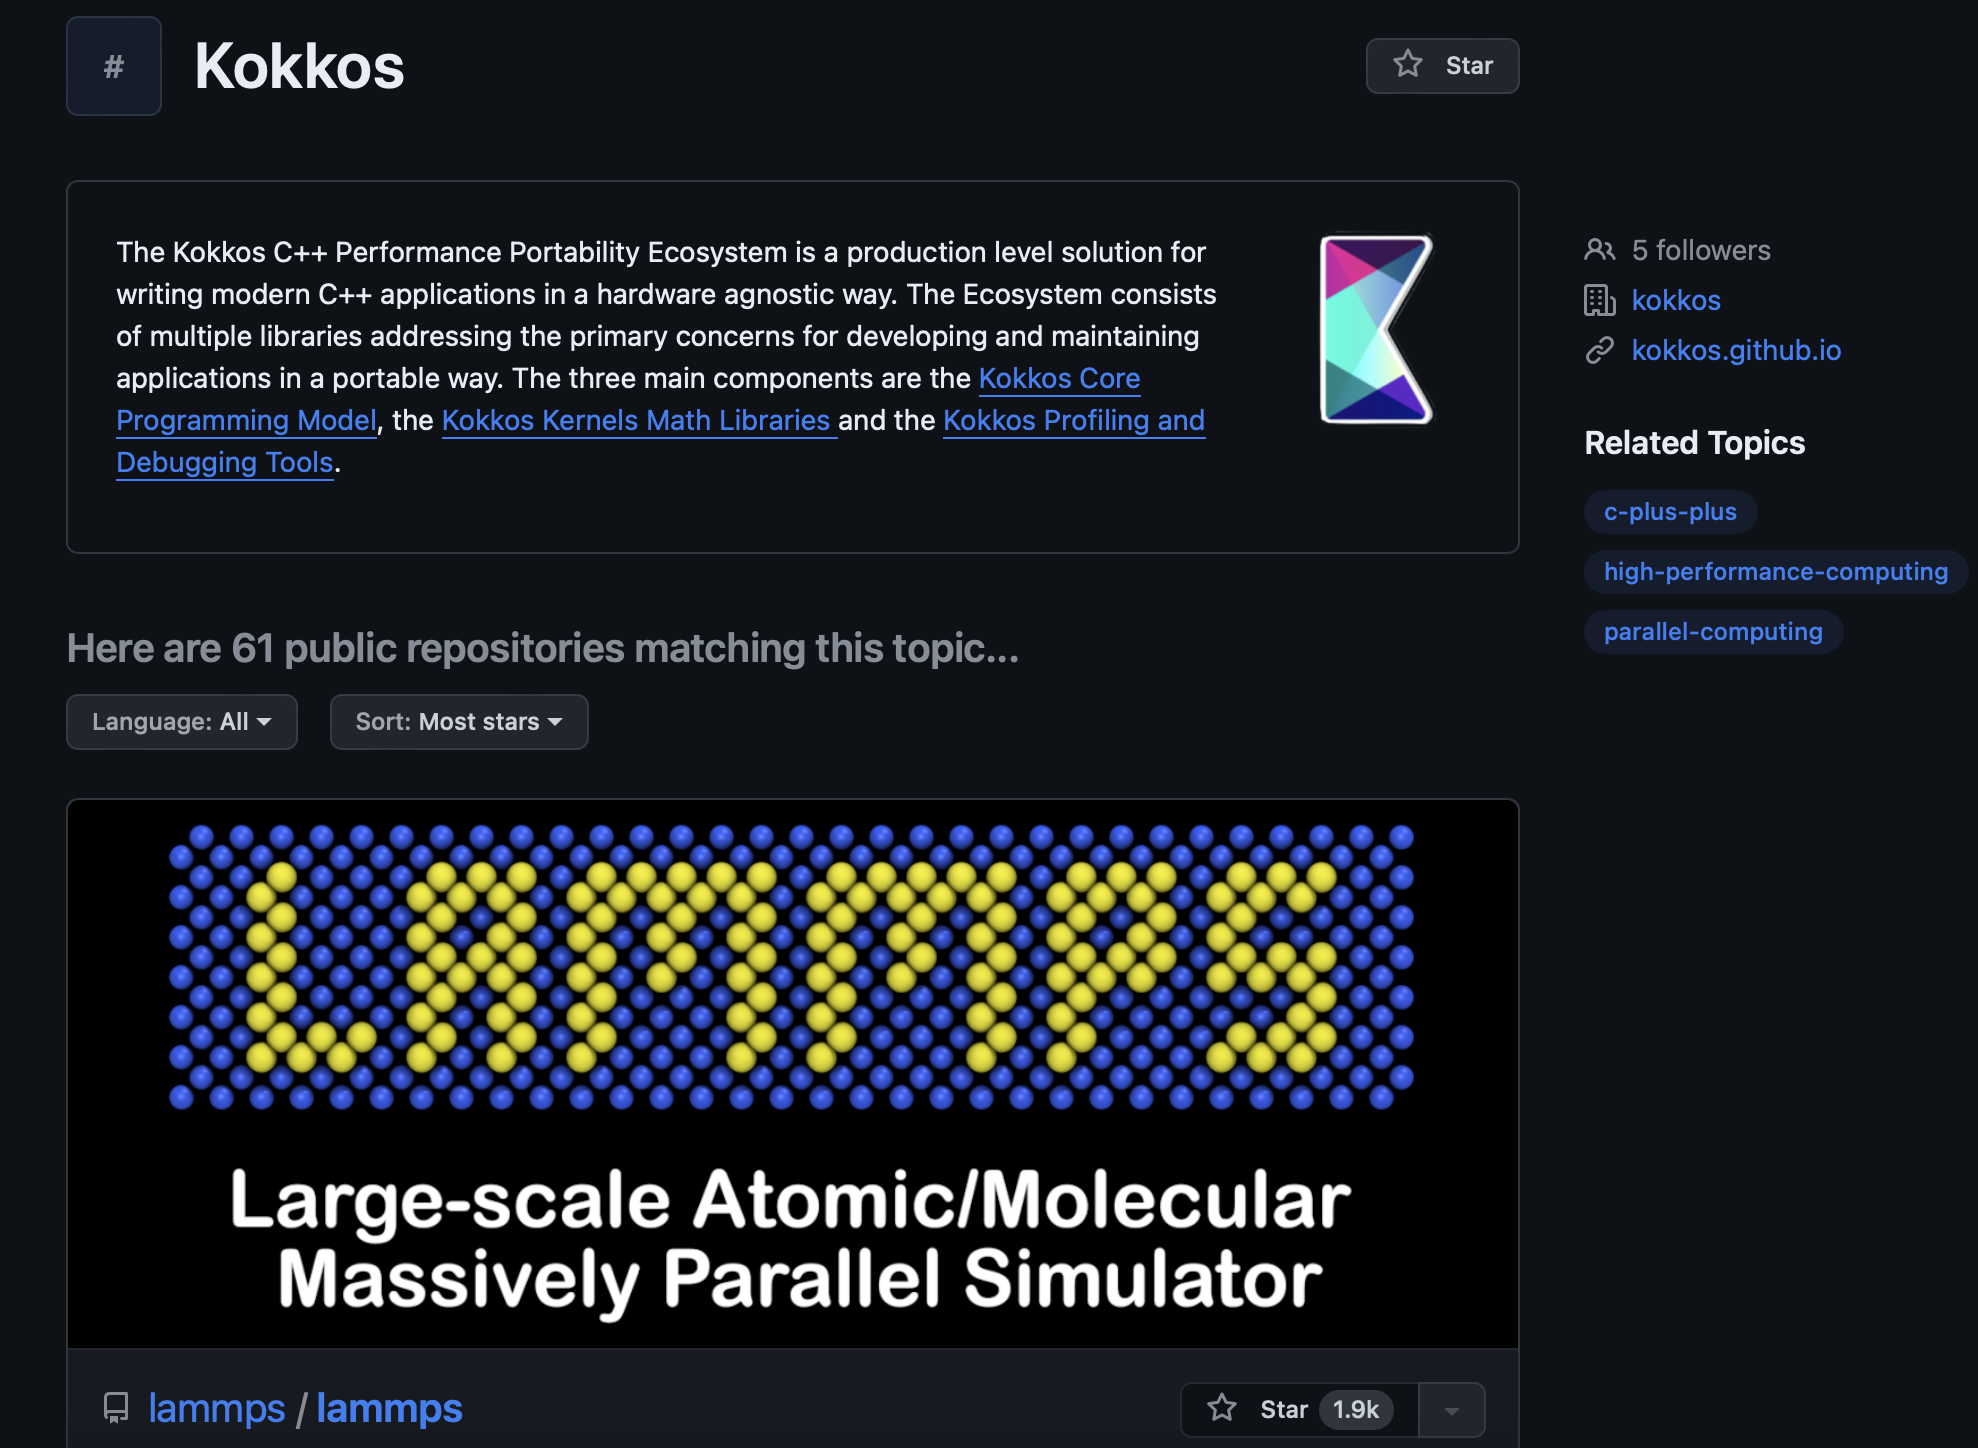
\includegraphics[width=0.9\textwidth]{4_2/kokkos-topic}
\end{frame}

%==========================================================================

\begin{frame}[fragile]

  {\Huge Backend Updates}

  \vspace{10pt}

\end{frame}


%==========================================================================

% Examples

% note: always keep the [fragile] for your frames!

%\begin{frame}[fragile]{Title}
%  Contents
%\end{frame}

%==========================================================================
\begin{frame}[fragile]{CUDA and SYCL}
  \begin{itemize}
    \item CUDA: Add support for AMPERE87 architecture (Jetson Orin Nano)
    \item CUDA: Support RDC with Clang 17+ and use new offload driver
    \item SYCL: Add support for Intel DG2 GPUs such as the Arc Alchemist GPUs
    \item SYCL: Allow using non-trivially-copyable comparators with oneDPL
  \end{itemize}
\end{frame}

%==========================================================================

\begin{frame}[fragile]{Improve half float performance for CUDA and SYCL backends}
  \begin{itemize}
    \item CUDA AND SYCL: Directly use the available fp16 mathematical function instead of casting back and forth to fp32
  \end{itemize}
  \begin{tikzpicture}
    \begin{axis}[
        width  = 0.85*\textwidth,
        height = 0.75*\textheight,
        major x tick style = transparent,
        ybar=2*\pgflinewidth,
        bar width=14pt,
        ymajorgrids = true,
        ylabel = {Exec time (µs)},
        symbolic x coords={Memory Bound Kernel, Compute Bound Kernel},
        xtick = data,
        scaled y ticks = false,
        enlarge x limits=0.25,
        ymin=0,
        legend style={at={(0.3,0.75)},anchor=west},
    ]
        \addplot
            coordinates {(Memory Bound Kernel, 32) (Compute Bound Kernel, 102)};

        \addplot
            coordinates {(Memory Bound Kernel, 15.8) (Compute Bound Kernel, 102)};

        \addplot
            coordinates {(Memory Bound Kernel, 14.7) (Compute Bound Kernel, 63)};

        \legend{float 32, fp16 old, fp16 new}
    \end{axis}
\end{tikzpicture}
\end{frame}

% Bench details:
% - NVidia A100
% - 2^20 (1 million) elements
% - Memory bound kernel is doing:
% tmp = init(i);
% res(i) = sqrt(cos(tmp) + sin(tmp));
% - Compute bound is doing 16 time the work of Memory Bound

%==========================================================================

\begin{frame}[fragile]{OpenMPTarget}
  \begin{itemize}
      \item Remove support for non-llvm compilers as part of the strategy to only support LLVM compilers in the backend.
      \item LLVM compilers support extensions to OpenMP directives on GPU that allow \textit{grid} style kernel launches making it more suitable for GPUs and avoiding the overhead of OpenMP's fork-join model.
  \end{itemize}
\end{frame}

%==========================================================================

%==========================================================================

\begin{frame}[fragile]

  {\Huge Build Systems Updates}

  \vspace{10pt}

\end{frame}

%==========================================================================

% Examples

% note: always keep the [fragile] for your frames!

\begin{frame}[fragile]{New build system features}
  \begin{itemize}
    \item Add support for Zen 4 AMD microarchitecture (\texttt{Kokkos\_ARCH\_ZEN4})
    \item Enable NVIDIA Grace architecture with NVHPC (\texttt{Kokkos\_ARCH\_ARMV9\_GRACE})
    \item Support static library builds via \texttt{CMAKE\_CUDA\_RUNTIME\_LIBRARY=static} when using CUDA as CMake language
  \end{itemize}

\end{frame}

%==========================================================================


%==========================================================================


%==========================================================================

\begin{frame}[fragile]

  {\Huge SIMD}

  \vspace{10pt}

  {\large Portable vector intrinsic types.}

  \vspace{20pt}

  \textbf{Learning objectives:}
  \begin{itemize}
    \item {How to use SIMD types to improve vectorization.}
    \item {SIMD Types as an alternative to ThreadVector loops.}
    \item {SIMD Types to achieve outer loop vectorization.}
  \end{itemize}

  \vspace{-20pt}

\end{frame}

%==========================================================================

\begin{frame}[fragile]{Vectorization In Kokkos}

   So far there were two options for achieving vectorization: 

\begin{itemize}
  \item{{\textbf{Hope For The Best}}: Kokkos semantics make loops inherently vectorizable, sometimes the compiler figures it even out.}
  \item{{\textbf{Hierarchical Parallelism}}: {\texttt{TeamVectorRange}} and {\texttt{ThreadVectorRange}} help the compiler with hints such as {\texttt{\#pragma ivdep}} or {\texttt{\#pragma omp simd}}}.
\end{itemize}

   \vspace{3pt}

  These strategies do run into limits though:

\begin{itemize}
  \item{Compilers often do not vectorize loops on their own.}
  \item{An optimal vectorization strategy would require \emph{outer-loop vectorization}.}
  \item{Vectorization with \texttt{TeamVectorRange} sometimes requires artifically introducing an additional loop level.}
\end{itemize}
\end{frame}

\begin{frame}[fragile]{Outer-Loop Vectorization}

   A simple scenario where for outer-loop vectorization:
	\vspace{-3pt}
  \begin{code}[linebackgroundcolor={},keywords={for,int}]
  for(int i=0; i<N; i++) {
    // expect K to be small odd 1,3,5,7 for physics reasons
    for(int k=0; k<K; k++) b(i) += a(i,k);
  }
  \end{code}

  Vectorization the \texttt{K}-Loop is not profitable:
  \begin{itemize}
	  \item{It is a short reduction.}
	  \item{Remainders will eat up much time.}
  \end{itemize}
	\vspace{5pt}

  Using \texttt{ThreadVectorRange} is cumbersome and requires split of \texttt{N}-Loop:

  \begin{code}[linebackgroundcolor={},keywords={parallel_for,for,int,TeamPolicy,ThreadVectorRange}]
parallel_for("VectorLoop",TeamPolicy<>(0,N/V,V),
  KOKKOS_LAMBDA ( const team_t& team ) {
  int i = team.league_rank() * V;
  for(int k=0; k<K; k++) 
    parallel_for(ThreadVectorRange(team,V), [&](int ii) {
      b(i+ii) += a(i+ii,k);
    });
});
    \end{code}
\end{frame}

\begin{frame}[fragile]{SIMD Types}
  
   To help with this situation and (in particular in the past) fix the lack of auto-vectorizing compilers \texttt{SIMD-Types} have been invented. They:
	\begin{itemize}
		\item{Are short vectors of scalars.}
		\item{Have operators such as \texttt{+=} so one can use them like scalars.}
		\item{Are compile time sized.}
		\item{Usually map directly to hardware vector instructions.}
	\end{itemize}
	
	\begin{block}{Important concept: SIMD Type}
		A SIMD variable is a \textbf{short vector} which acts like a scalar.
  \end{block}

	Using such a \texttt{simd} type one can simply achieve \emph{outer-loop} vectorization by using arrays of \texttt{simd} and dividing the loop range by its \emph{size}.
\end{frame}

\begin{frame}[fragile]{Outer-Loop Vectorization}

  Lets take a look back at the outer loop vectorization:
  \begin{code}[linebackgroundcolor={},keywords={for,int}]
  View<double*> b = ...
  View<double**> a = ...
  for(int i=0; i<N; i++) {
    // expect K to be small odd 1,3,5,7 for physics reasons
    for(int k=0; k<K; k++) b(i) += a(i,k);
  }
  \end{code}

  \pause
  Using SIMD types is conceptionally as simple as:
	\begin{itemize}
		\item Replace scalar type with SIMD type
		\item Adjust loop iteration count by SIMD length
	\end{itemize}

  \begin{code}[linebackgroundcolor={},keywords={for,int}]
  using simd_t = Kokkos::Experimental::simd<double>;
  View<simd_t*> b = ...
  View<simd_t**> a = ...
  int V = simd_t::size();
  for(int i=0; i<N/V; i++) {
    // expect K to be small odd 1,3,5,7 for physics reasons
    for(int k=0; k<K; k++) b(i) += a(i,k);
  }
  \end{code}
\end{frame}

\begin{frame}[fragile]{C++26 SIMD}
	The ISO C++ standard has data-parallel types (\texttt{SIMD}) (in \emph{C++26}):

  \begin{code}[linebackgroundcolor={},keywords={template,class,public,using}]
template< class T, class Abi >
class basic_simd {
public:
  using value_type = T;
  using abi_type   = Abi;
  using mask_type  = basic_simd_mask<sizeof(T), Abi>;

  static constexpr integral_constant<simd-size-type, ...> size {};
  constexpr T operator[] (simd-size-type) const;
  // Element-wise operators
};

// Element-wise non-member functions

  \end{code}

\end{frame}

\begin{frame}[fragile]{C++26 SIMD ABI}
One interesting innovation here is the \texttt{Abi} parameter allowing for different, hardware specific, implementations.

	\vspace{8pt}

The most important components of \texttt{basic\_simd} are:
\begin{itemize}
	\item{\textbf{scalar\_abi}: single element type.}
	\item{\textbf{native\_abi}: best fit for hardware.}
	\item{\textbf{fixed\_size$<$N$>$}: the width of the simd type.}
\end{itemize}

\pause
	\vspace{8pt}

	But \texttt{std::simd} doesn't support GPUs ...

	\pause
	\vspace{8pt}
	It also has other problems making it insufficient for our codes...
\end{frame}

\begin{frame}[fragile]{Kokkos SIMD}
   Just at Sandia we had at least \textbf{5} different SIMD types in use.

   \vspace{8pt}
   A unification effort was started with the goal of:
   \begin{itemize}
      \item{Match the proposed \texttt{std::simd} API as far as possible.}
      \item{Support GPUs.}
      \item{Can be used stand-alone or in conjunction with Kokkos.}
      \item{Replaces all current implementations at Sandia for SIMD.}
   \end{itemize}

\end{frame}

\begin{frame}[fragile]{Kokkos SIMD}
  As with the C++26 SIMD type, it takes a data type and ABI
  \begin{code}
     template <class T, class Abi>
     class basic_simd;
  \end{code}

  Supported ABIs are:
  \begin{itemize}
    \item \texttt{simd\_abi::scalar}: a single element
    \item \texttt{simd\_abi::$[$native\_$]$fixed\_size<N>}: a specific data-parallel type available on the architecture (e.g. \texttt{avx512\_fixed\_size})
  \end{itemize}

  But for convenience, a simplified alias for \texttt{basic\_simd} is available:
  \begin{code}
    template <class T, int N = /* native_simd_width */>
    using simd = basic_simd<...>;
  \end{code}

  This abstracts ABI and allows using the optimal native data-parallel width on the architecture

\end{frame}

\begin{frame}[fragile]{Exercise: Simple SIMD usage.}

  \textbf{Details}:
  \begin{small}
  \begin{itemize}
\item Location: \ExerciseDirectory{simd/Begin}
\item Include the \texttt{Kokkos\_SIMD.hpp} header.
\item Change the data type of the views to use \texttt{simd$<$double$>$}.
\item Create an unmanaged \texttt{View$<$double*$>$} of \texttt{results} using the \texttt{data()} function for the final reduction.  
\end{itemize}
  \end{small}

\begin{code}
  # Configure, build, and run
    cmake -Bbuilddir -DKokkos_ARCH_NATIVE=ON
    cmake --build builddir
    ./builddir/SIMD
\end{code}

	\vspace{-3pt}
\ul{\textbf{Things to try:}}
  \begin{small}
  \begin{itemize}
  \item Vary problem size (-N ...; -M ...)
  \item Compare behavior of scalar vs vectorized on CPU and GPU
  \end{itemize}
  \end{small}



\end{frame}

\begin{comment}
\begin{frame}[fragile]{The GPU SIMD Problem}
  The above exercise used a \textbf{scalar} simd type on the \textbf{GPU}.
  
	{\textbf Why wouldn't we use a fixed\_size instead?}

	\begin{itemize}
	   \item{Using a \texttt{fixed\_size} ABI will create a scalar of size \texttt{N} in each CUDA thread!}
	   \item{Loading a \texttt{fixed\_size} variable from memory would result in uncoalesced access.}
           \item{If you have correct layouts you get \texttt{outer-loop} vectorization implicitly on GPUs.}
	\end{itemize}

	\pause
	But what if you really want to use \textbf{warp}-level parallelization for SIMD types?

	\pause
	{\textbf We need \emph{two} SIMD types: a \emph{storage} type and a \emph{temporary} type!}
\end{frame}

\begin{frame}[fragile]{cuda\_warp ABI}
  \begin{block}{Important concept: simd::storage\_type}
    Every \texttt{simd$<$T,ABI$>$} has an associated \texttt{storage\_type} typedef.
  \end{block}

  To help with the GPU issue we split types between \textbf{storage} types used for \texttt{Views}, and \textbf{temporary} variables.

  \begin{itemize}
	  \item{Most \texttt{simd::simd} types will just have the same \texttt{storage\_type}.}
	  \item{\texttt{simd$<$T,cuda\_warp$<$N$> >$} will use warp level parallelism.}
	  \item{\texttt{simd$<$T,cuda\_warp$<$N$> >$::storage\_type} is different though!}
	  \item{Used in conjunction with \texttt{TeamPolicy}.}
  \end{itemize}
\end{frame}

\begin{frame}[fragile]{cuda\_warp ABI}
\textbf{Illustrating difference between \texttt{pack} and \texttt{cuda\_warp}}


      \begin{code}[linebackgroundcolor={},keywords={simd,parallel_for,using}]
using ABI = ... ;
View<simd<double,ABI::storage_type> A(...);
parallel_for(TeamPolicy<>(N,AUTO,V), 
 KOKKOS_LAMBDA(const teamt_t& team) {
  int i = team.league_rank()*team.team_size()+team.team_rank();
  simd<double,ABI> tmp = A(i);
});
       \end{code}
  \begin{columns}[]
    \begin{column}{.5\textwidth}
      \begin{code}[linebackgroundcolor={},keywords={pack,using}]
using ABI = pack<8>; int V=1;
\end{code}

       \includegraphics[width=0.75\textwidth]{figures/simd-fixedsize} 

    \end{column}
    \begin{column}{.5\textwidth}
      \begin{code}[linebackgroundcolor={},keywords={cuda_warp,using}]
using ABI = cuda_warp<8>; int V=8;
\end{code}

       \includegraphics[width=0.75\textwidth]{figures/simd-warp} 

    \end{column}
  \end{columns}
\end{frame}

\begin{frame}[fragile]{cuda\_warp ABI}

Example of using \texttt{storage\_type}:

\begin{code}[linebackgroundcolor={},keywords={template,class,simd,simd_storage,TeamPolicy,TeamThreadRange,public,using}]
// Using cuda_warp abi
using simd_t = simd::simd<T,simd::simd_abi::cuda_warp<V> >;
// Define simd_storage type
using simd_storage_t = simd_t::storage_type;
// Allocate memory
View<simd_storage_t**> data("D",N,M); // will hold N*M*V Ts

// Launch Loop with vectorlength V
parallel_for("Loop", TeamPolicy<>(N,M,V), 
  KOKKOS_LAMBDA(const team_t& team) {
    int i = team.league_rank();
    parallel_for(TeamThreadRange(team,M), [&](int j) {
      // Load storage type into internal type;
      simd_t tmp = data(i,j);
      // Do something with it
      tmp *= 2.0;
      // write values back
      data(i,j) = tmp;
      // or inline:
      // data(i,j) = 2.0*simd_t(data(i,j));
  }); 
});
\end{code}

\end{frame}


\begin{frame}[fragile]{Exercise: SIMD storage usage.}

  \textbf{Details}:
  \begin{small}
  \begin{itemize}
\item Location: \ExerciseDirectory{simd\_warp/Begin}
\item Include the \texttt{simd.hpp} header.
\item Change the data type of the views to use \texttt{simd::simd$<$double,simd::simd\_abi:cuda\_warp$<32>>$::storage\_type}.
\item Create an unmanaged \texttt{View$<$double*$>$} of \texttt{results} using the \texttt{data()} function for the final reduction.  
\item Use inside of the lambda the \texttt{simd::simd$<$double,simd::simd\_abi:cuda\_warp$<32>>$} as scalar type.
\end{itemize}
  \end{small}

\begin{code}
   # Compile for GPU
   make -j KOKKOS_DEVICES=Cuda
   # Run on GPU
   ./simd.cuda
\end{code}

\end{frame}
\end{comment}

\begin{frame}[fragile]{Advanced SIMD Capabilities}

Kokkos SIMD supports math operations:
\begin{itemize}
  \item{Common stuff like \texttt{abs}, \texttt{sqrt}, \texttt{exp}, ...}
\end{itemize}

\vspace{8pt}
It also supports masking:

	\begin{code}
// Scalar code with condition:
for(int i=0; i<N; i++) {
  if( a(i) < 100.0 ) b(i) = a(i);
  else b(i) = 100.0;
}

// Becomes
using simd_t      = simd<double>;
using simd_mask_t = simd_t::mask_type;
   
for(int i=0; i<N/V; i++) {
  simd_t threshold(100.0), a_i(a_v(i));
  simd_mask_t is_smaller = threshold<a_i;

  b_v(i) = condition(is_smaller,a_i,threshold);
}
\end{code}
\end{frame}

\begin{frame}[fragile]{SIMD Summary}
	\begin{itemize}
		\item{SIMD types help vectorize code.}
		\item{In particular for \textbf{outer-loop} vectorization.}
		\item{There are \textbf{storage} and \textbf{temporary} types.}
		\item{Masking is supported too.}
	\end{itemize}
\end{frame}
%==========================================================================

\begin{frame}[fragile]{Half-precision floating-point types updates}

\texttt{half\_t} (since 3.3) and \texttt{bhalf\_t} (since 3.6) defined in
namespace \texttt{Kokkos::Experimental::}

\begin{itemize}
\item Specialized numeric traits for \texttt{half\_t} and \texttt{bhalf\_t}
  \begin{itemize}
  \item Half-precision types still cannot appear in constant
  expressions
  \item Distinguished values are of an implementation-defined type
  convertible to half-precision
  \end{itemize}
\begin{code}
static_assert(
  !std::is_same_v<decltype(infinity_v<half_t>), half_t> &&
  std::is_convertible_v<decltype(infinity_v<half_t>, half_t>
);
\end{code}
\item Added mathematical functions overloads
  \begin{itemize}
  \item Currently falling back to \texttt{float} and not actually using
        intrinsics...
  \end{itemize}
\item Implemented support for mixed comparisons
\begin{code}
x < 0.f  // OK
0.f < x  // error before but fine since 4.2
\end{code}
\end{itemize}
\end{frame}

\begin{frame}[fragile]{\texttt{Kokkos::printf}}
\begin{itemize}
\item Defined in header \texttt{<Kokkos\_Printf.hpp>} which is included from
      \texttt{<Kokkos\_Core.hpp>}
\item Prints formated output to the standard output stream
\item Calling \texttt{Kokkos::printf()} from a kernel may affect register usage
      and affect performance.
\end{itemize}
\begin{code}[keywords={printf}]
#include <Kokkos_Core.hpp>

int main(int argc, char* argv[]) {
    Kokkos::initialize(argc, argv);
    Kokkos::parallel_for(4, KOKKOS_LAMBDA(int i) {
        Kokkos::printf("hi from thread %d\n", i);
    });
    Kokkos::finalize();
}
\end{code}
\end{frame}

\begin{frame}[fragile]{Serial execution space instances}
\begin{itemize}
\item Allow creating non-default \texttt{Serial} exec space instances
\item New constructor taking \texttt{NewInstance} tag as argument
\begin{code}[keywords={NewInstance}]
Kokkos::Serial e1(Kokkos::NewInstance());

auto e2 = Kokkos::Experimental::partition_space(
  Kokkos::DefaultHostExecutionSpace(), 1)[0]; // better
\end{code}
\item Thread safe since 3.5 but kernels were effectively serialized
\item Now enabling overlap of computation on distinct instances
\end{itemize}
\end{frame}

\begin{frame}[fragile]{Serial execution space instances}
\begin{code}[keywords={NewInstance}]
#include <Kokkos_Core.hpp>
#include <thread>

template <class Exec> void foo(Exec exec) {
  parallel_for("foo", RangePolicy<Exec>(exec, 0, 3),
    KOKKOS_LAMBDA(int i) { printf("just doin my job %d\n", i); });
}

template <class Exec> void bar(Exec exec) { /* ... */ }

int main(int argc, char *argv[]) {
  Kokkos::ScopeGuard kenv(argc, argv);
  using Exec = Kokkos::DefaultHostExecutionSpace;
  auto instances = Kokkos::Experimental::partition_space(
    Exec(), 1, 1);
  std::thread t0(foo<Exec>, instances[0]);
  std::thread t1(bar<Exec>, instances[1]);
  t0.join();
  t1.join();
  return 0;
}
\end{code}

\end{frame}


\begin{frame}[fragile]{Kokkos Std Algorithms: added support for team-level}

\begin{itemize}
\item Defined in header \texttt{<Kokkos\_StdAlgorithms.hpp>}
\item Extended API with a new overload for team-level support

\begin{code}[keywords={sort}]
template <class TeamHandleT, ...>
KOKKOS_FUNCTION
/*ret type*/ algo_name(const TeamHandleT& /*teamHandle*/,
                       /*view(s) or iterators*/,
                       /*extra*/);
\end{code}

\item \texttt{teamHandle}: given in parallel region when using TeamPolicy

\item \texttt{view(s)}: rank-1, \texttt{LayoutLeft,Right,Stride}

\item \texttt{iterators}: must be random access (use \texttt{Kokkos::Experimental::begin,end,cbegin,cend})

\item views and iterators must be accessible from \texttt{space} or from the space associated with \texttt{teamHandle}

\item \texttt{extra}: parameters that are specific to the algorithm

\end{itemize}

\end{frame}


\begin{frame}[fragile]{\texttt{Kokkos::sort} accepts a custom comparison functor}

\begin{itemize}
\item Defined in header \texttt{<Kokkos\_Sort.hpp>}
\item Two new overloads to support a custom comparator.

\begin{code}[keywords={sort}]
template <class ExecSpace, class ViewType, class CompType>
void sort(const ExecSpace& exespace,     // (1)
          const ViewType & view,
          const CompType & comparator);

template <class ViewType, class CompType>
void sort(const ViewType & view,         // (2)
          const CompType & comparator);
\end{code}

\item \texttt{view} must be rank-1 with \texttt{LayoutLeft}, \texttt{LayoutRight}, or \texttt{LayoutStride}
  and must be accessible from \texttt{exespace}

\item (1) is potentially asynchronous
\item (2) calls (1) using the \texttt{view}'s execution space, and fences
\end{itemize}

\end{frame}


\begin{frame}[fragile]{\texttt{Kokkos::sort} accepts a custom comparison functor}

\begin{itemize}
\item \texttt{comparator} must be callable from the execution space passed
\item \texttt{comparator} must be callable with two arguments \texttt{a,b} of type (possible const-qualified) \texttt{value\_type}, where \texttt{value\_type} is the non-const value type of the \texttt{view}.
\item Snippet:
\begin{code}[keywords={sort}]
struct MyComp {
KOKKOS_FUNCTION bool operator()(int a, int b) const{
  // return true if a is less than b,
  // according to some, potentially non-trivial logic
}

Kokkos::View<int*> v("v", 1000);
Kokkos::sort(v, MyComp());
\end{code}

\end{itemize}

\end{frame}


%==========================================================================
\begin{frame}[fragile]

  {\huge \texttt{parallel\_scan}: new overload for nested policies with return value}

  \vspace{10pt}

  \textbf{Content:}
  \begin{itemize}
    \item API
    \item Example
  \end{itemize}

\end{frame}


%==========================================================================
\begin{frame}[fragile]{\texttt{parallel\_scan}: new overload API}

\begin{itemize}
\item New overload with return value for nested policies

\hspace{-0.8cm}
\begin{code}[keywords={parallel_scan}]
template<class ExecPolicy, class FunctorType, class ReturnType>
KOKKOS_FUNCTION
Kokkos::parallel_scan(const ExecPolicy &policy,
                      const FunctorType &functor,
                      ReturnType &return_value);
\end{code}

\vspace{4pt}
\item Valid policies: \texttt{ThreadVectorRange}, \texttt{TeamThreadRange}

\vspace{4pt}
\item \texttt{return\_value} is {\bf overwritten}

\vspace{4pt}
\item Only valid inside a parallel region executed via \texttt{TeamPolicy} or \texttt{TaskTeam}.

\vspace{4pt}
\item \texttt{ReturnType} must be compatible with the type of functor

\end{itemize}

\end{frame}


%==========================================================================
\begin{frame}[fragile]{\texttt{parallel\_scan}: new overload's representative snippet}

\hspace{-1.1cm}
\begin{code}[keywords={parallel_scan, TeamThreadRange, TeamPolicy}]
  template<class ViewType, class TeamHandleType>
  struct Functor{
    ViewType m_view;

    KOKKOS_FUNCTION void operator()(const TeamHandleType& handle) const{
      const auto leagueRank = handle.league_rank();
      // ...
      int accum;
      Kokkos::parallel_scan(
         Kokkos::TeamThreadRange(handle, 0, m_view.extent(1)),
         KOKKOS_LAMBDA(int i, value_type& val, const bool final) {
           val += m_view(leagueRank, i);
           if (final) { // do something }
         }, accum);
    }};

  using view_t       = Kokkos::View<int**>;
  using policy_t     = Kokkos::TeamPolicy<>;
  using team_hande_t = typename policy_t::member_type;
  view_t v("v", numRows, numCols);
  Kokkos::parallel_for(policy_t(numRows, Kokkos::AUTO),
                       Functor<view_t, team_hande_t>(...));
\end{code}

\end{frame}


\begin{frame}[fragile]{Miscellaneous}
\begin{itemize}
  \item Add \texttt{Kokkos::Profiling::ScopedRegion}
    \begin{code}	
     double myfunction()
     {
      Kokkos::Profiling::ScopedRegion region("foo");
      if (..)
        return bar;
      else
        return eval();
     }
    \end{code}
  \item Add support for \texttt{View::rank[\_dynamic]()}
  \item Detect incompatible relocatable device code mode to prevent ODR violations
  \item Add (experimental) support for 32-bit Darwin and PPC
  \item Add missing half and bhalf specialization of the infinity numeric trait
\end{itemize}
\end{frame}

\begin{frame}[fragile]{Miscellaneous}
\begin{itemize}
  \item Add \texttt{is\_dual\_view} trait and align template parameters with regular view
  \item Allow templated functors in \texttt{parallel\_for},
  \texttt{parallel\_reduce}, and \texttt{parallel\_scan}
  \item Define \texttt{KOKKOS\_COMPILER\_INTEL\_LLVM} and only define at most one
  \texttt{KOKKOS\_COMPILER*} macro
\end{itemize}
\end{frame}

%==========================================================================

\begin{frame}[fragile]

  {\Huge Bug Fixes}

  \vspace{10pt}

\end{frame}

%==========================================================================

% Examples

% note: always keep the [fragile] for your frames!

%\begin{frame}[fragile]{Example list}
%  \begin{itemize}
%      \item Item 1
%      \item Item 2 with some \texttt{code}
%      \begin{itemize}
%        \item Sub-item 2.1
%        \item Sub-item 2.2
%      \end{itemize}
%  \end{itemize}
%\end{frame}

%\begin{frame}[fragile]{Example code}
%    \begin{code}[keywords={std}]
%        #include <iostream>
%        
%        int main() {
%            std::cout << "hello world\n";
%        }
%    \end{code}
%\end{frame}

%\begin{frame}[fragile]{Example table}
%    \begin{center}
%        \begin{tabular}{l|l}
%            a & b \\\hline
%            c & d
%        \end{tabular}
%    \end{center}
%\end{frame}

%==========================================================================


%==========================================================================

%==========================================================================

\begin{frame}[fragile]

  {\Huge Deprecations and other breaking changes}

  \vspace{10pt}

\end{frame}


\begin{frame}[fragile]{Intel Classic Compiler}
  \begin{itemize}
    \item Intel has long since deprecated Intel Classic (since around 2022), and removed from oneAPI 2024.0 release
    \item In order to focus on newer compilers, and reduce maintenance burden, we have \textbf{removed} support for Intel Classic (oneAPI Intel/icpx still supported of course!)
  \end{itemize}
\end{frame}


\begin{frame}[fragile]{DualView changes}
  \textbf{Deprecate} direct access to \texttt{d\_view} and \texttt{h\_view}
  \begin{itemize}
    \item Modifying the allocations in d\_view and h\_view directly is dangerous, especially if \texttt{modify} and \texttt{sync} are skipped
    \item Use \texttt{view\_host()} and \texttt{view\_device()} instead
    \item These two functions return by value with deprecated code enabled and by const reference otherwise. This might have perfomance implications if used extensively, e.g., in loop bounds.
  \end{itemize}
\end{frame}


\begin{frame}[fragile]{Experimental SIMD changes}
  \begin{itemize}
    \item \texttt{native\_simd}, \texttt{native\_simd\_mask} \textbf{deprecated} to align with the C++26 standard
    \item \textbf{Removed} Obtaining a reference from \texttt{*simd*::operator[]} to align with the C++26 Standard
    \item \textbf{Changed} the return type of \texttt{Kokkos::Experimental::*simd*::operator==} and \texttt{operator!=} to return SIMD masks instead of \texttt{bool}
    \begin{itemize}
      \item If you want old behavior, use \texttt{all\_of(a == b)}
    \end{itemize}
  \end{itemize}
\end{frame}

\begin{frame}[fragile]{Additional Deprecations and Removals}
  \begin{itemize}
    \item Already discussed deprecating the Makefile
    \item StaticCrsGraph is \textbf{moved} to Kokkos Kernels and \textbf{deprecated} in Core
    \begin{itemize}
      \item See \url{https://github.com/kokkos/kokkos-kernels/pull/2419}
      \item Symbol is in Kernels under \texttt{KokkosSparse::StaticCrsGraph}
    \end{itemize}
  \end{itemize}
\end{frame}
%==========================================================================

% Examples

% note: always keep the [fragile] for your frames!

%\begin{frame}[fragile]{Example list}
%  \begin{itemize}
%      \item Item 1
%      \item Item 2 with some \texttt{code}
%      \begin{itemize}
%        \item Sub-item 2.1
%        \item Sub-item 2.2
%      \end{itemize}
%  \end{itemize}
%\end{frame}

%\begin{frame}[fragile]{Example code}
%    \begin{code}[keywords={std}]
%        #include <iostream>
%        
%        int main() {
%            std::cout << "hello world\n";
%        }
%    \end{code}
%\end{frame}

%\begin{frame}[fragile]{Example table}
%    \begin{center}
%        \begin{tabular}{l|l}
%            a & b \\\hline
%            c & d
%        \end{tabular}
%    \end{center}
%\end{frame}

%==========================================================================


%==========================================================================

\begin{frame}[fragile]{Deprecations}
\begin{itemize}
\item Deprecated \texttt{Kokkos::vector}
\item Use \texttt{std::aligned\_alloc} for all host allocations
\begin{itemize}
\item Removed code that performed allocations with other mechanisms
\item Deprecated \texttt{PosixMemAlign}, \texttt{PosixMMap},
      \texttt{IntelMMAlloc} enumerators from
      \texttt{RawMemoryAllocationFailure::AllocationMechanism}
      which is defined in \texttt{Kokkos::Experimental::}
\item Deprecated the \texttt{HostSpace::AllocationMechanism} enumeration and
      the \texttt{HostSpace(AllocationMechanism)} explicit constructor
\end{itemize}
\end{itemize}
\end{frame}



%==========================================================================

\begin{frame}[fragile]

  \vspace{10pt}

  \textbf{How to Get Your Fixes and Features into Kokkos}
  \newline
  \begin{itemize}
    \item Fork the Kokkos repo (https://github.com/kokkos/kokkos)
    \item Make topic branch from \textit{develop} for your code
    \item Add tests for your code
    \item Create a Pull Request (PR) on the main project \textit{develop}
    \item Update the documentation (https://github.com/kokkos/kokkos-core-wiki) if your code changes the API
    \item Get in touch if you have any questions (https://kokkosteam.slack.com)
  \end{itemize}

\end{frame}

%==========================================================================

\end{document}
